\section{Análise exploratória}\label{sec:rn_eda}

\rnAprovados\% dos pedidos foram aprovados, cerca de \rnRazaoClasses{} aprovado para cada rejeitado: a base é moderadamente desbalanceada, e a acurácia sozinha engana, porque responder sempre ``aprovado'' já acerta \rnAprovados\%. Esse é o piso. Um atributo domina os demais: o score de crédito tem correlação de \rnCorrScore{} com a aprovação, enquanto o prazo tem \rnCorrPrazo{} e os outros nove ficam perto de zero. Os valores em dinheiro são redundantes entre si: a renda anual tem correlação de \rnCorrRendaValor{} com o valor do empréstimo e de \rnCorrRendaLuxo{} com os bens de luxo (Figura~\ref{fig:rn_corr}).

\begin{figure}[ht]
\centering
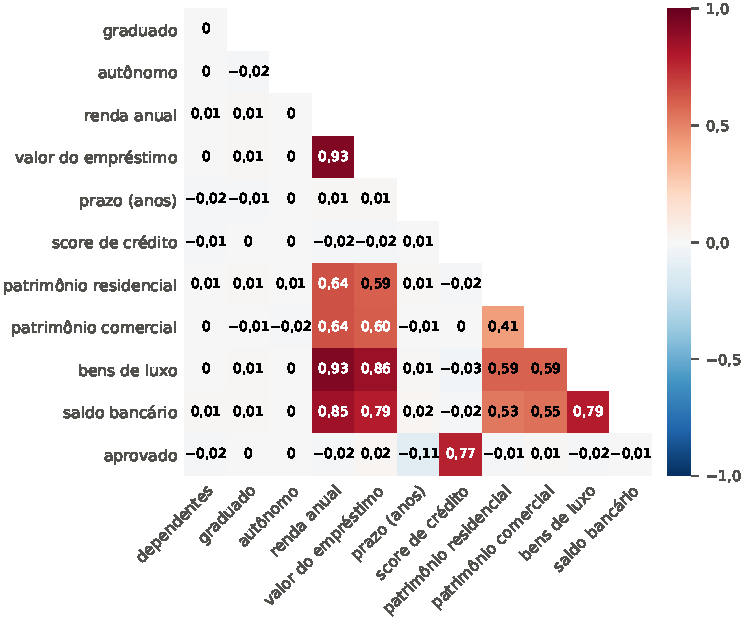
\includegraphics[width=.8\textwidth]{figures/rn_correlacao.pdf}
\caption{Correlação de Pearson entre os 11 atributos e a aprovação, na base inteira (\rnLinhas{} pedidos). Só o score de crédito se relaciona fortemente com a aprovação; os valores em dinheiro se correlacionam entre si e quase nada com o alvo.}
\label{fig:rn_corr}
\end{figure}

A Figura~\ref{fig:rn_score} mostra a forma dessa relação, e ela não é gradual: abaixo de 550 pontos, cerca de \rnAprovAbaixo\% dos pedidos são aprovados, em qualquer faixa; a partir de 550, \rnAprovAcima\%. A regra ``aprovar se o score for de pelo menos 550'' acerta \rnRegraBase\% da base. Os aprovados abaixo de 550 têm todos prazo de 2 ou 4 anos (\rnAprovPrazoDois\% e \rnAprovPrazoQuatro\% de aprovação nesses prazos); com prazos maiores, nenhum pedido abaixo de 550 foi aprovado. Os rótulos seguem, portanto, quase uma regra explícita: um degrau no score, com uma exceção para prazos curtos.

\begin{figure}[ht]
\centering
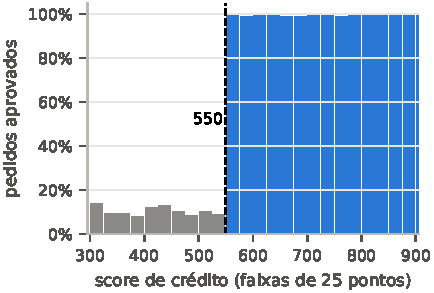
\includegraphics[width=.55\textwidth]{figures/rn_aprovacao_score.pdf}
\caption{Proporção de pedidos aprovados por faixa de 25 pontos de score de crédito. A linha tracejada marca 550.}
\label{fig:rn_score}
\end{figure}

A base parece sintética. O score e a renda se distribuem de forma quase uniforme: os quartis do score são 453, 600 e 748, contra 450, 600 e 750 de uma distribuição uniforme entre 300 e 900. Escolaridade e autônomo se dividem quase meio a meio. Com dados de crédito reais, seriam esperadas distribuições concentradas e uma relação mais gradual entre o score e a aprovação. Isso limita o alcance das conclusões (Seção~\ref{sec:limitacoes}).
